\documentclass[12pt,onecolumn]{article}


\usepackage{float}
\usepackage{mathtools}
\usepackage[russian]{babel}
\everymath{\displaystyle}

\usepackage[usenames]{color}
\usepackage{colortbl}

\usepackage{geometry}
\geometry{
  a4paper,
  top=15mm, 
  right=10mm, 
  bottom=15mm, 
  left=10mm
}

\begin{document}

\begin{center}
    Санкт-Петербургский Национальный Исследовательский\\ 
    Университет ИТМО\\
    Факультет Программной Инженерии и Компьютерной Техники\\
    % \includegraphics{itm.jpg}
\end{center}
\vspace{1cm}


\begin{center}
    \large \textbf{Вариант №31205}\\
    \textbf{Лабораторная работа №6}\\
    по дисциплине\\
    \textbf{\textit{'Программирование'}}
\end{center}

\vspace{3cm}
\begin{flushright}
  Выполнил Студент  группы P3118: \\
  \textbf{Михеев Илья Романович}\\
  Преподаватель: \\
  \textbf{Кулинич Ярослав Владимирович}\\
\end{flushright}

\vspace{14cm}
\begin{center}
    г. Санкт-Петербург\\
    2023г.
\end{center}

\newpage

\tableofcontents

\vspace{1cm}

\section{Текст задания}
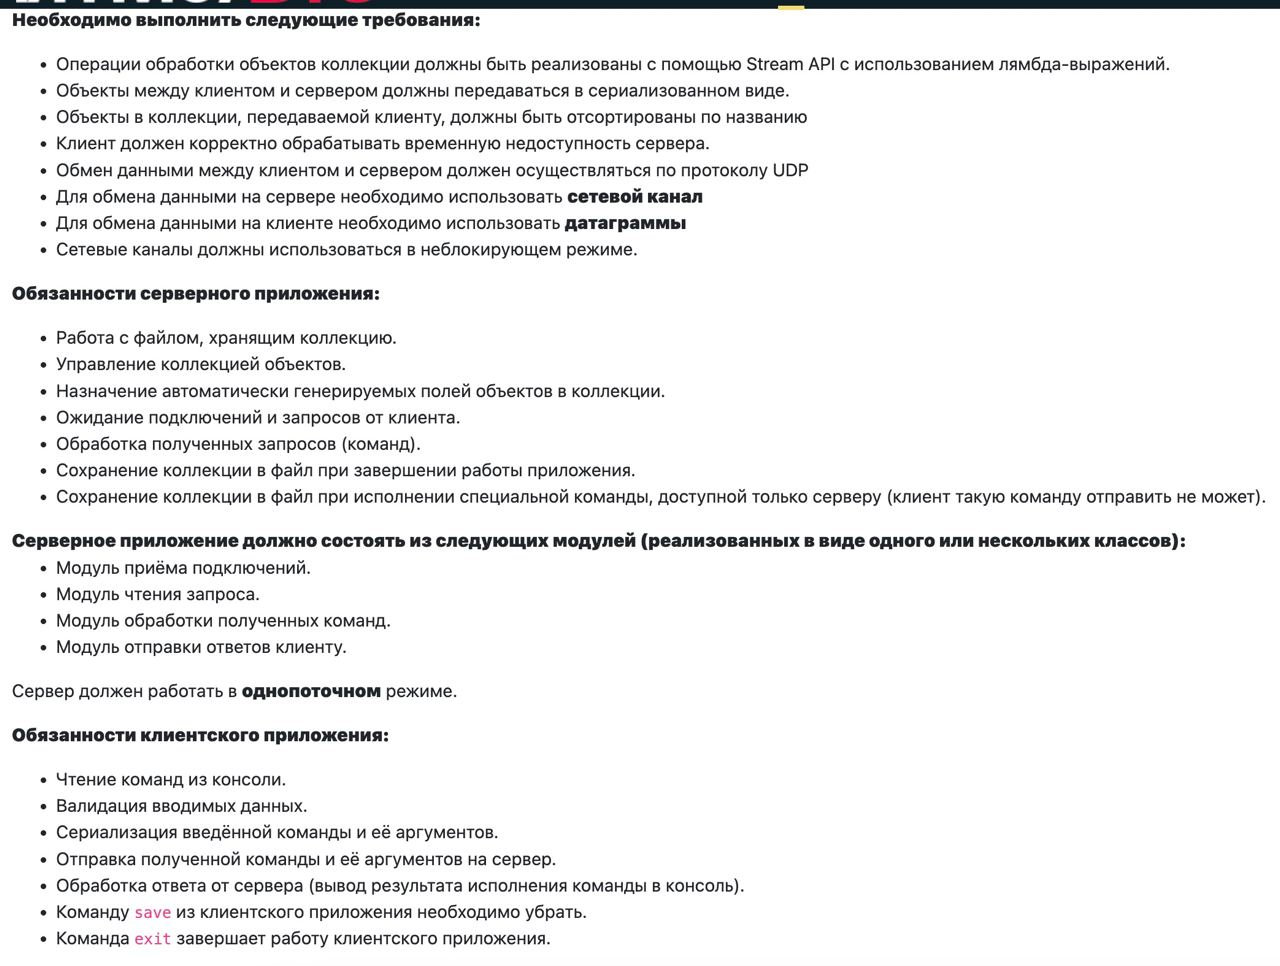
\includegraphics[width=\columnwidth]{imgs/lab6_task1.jpg}

\section{Диаграмма классов}
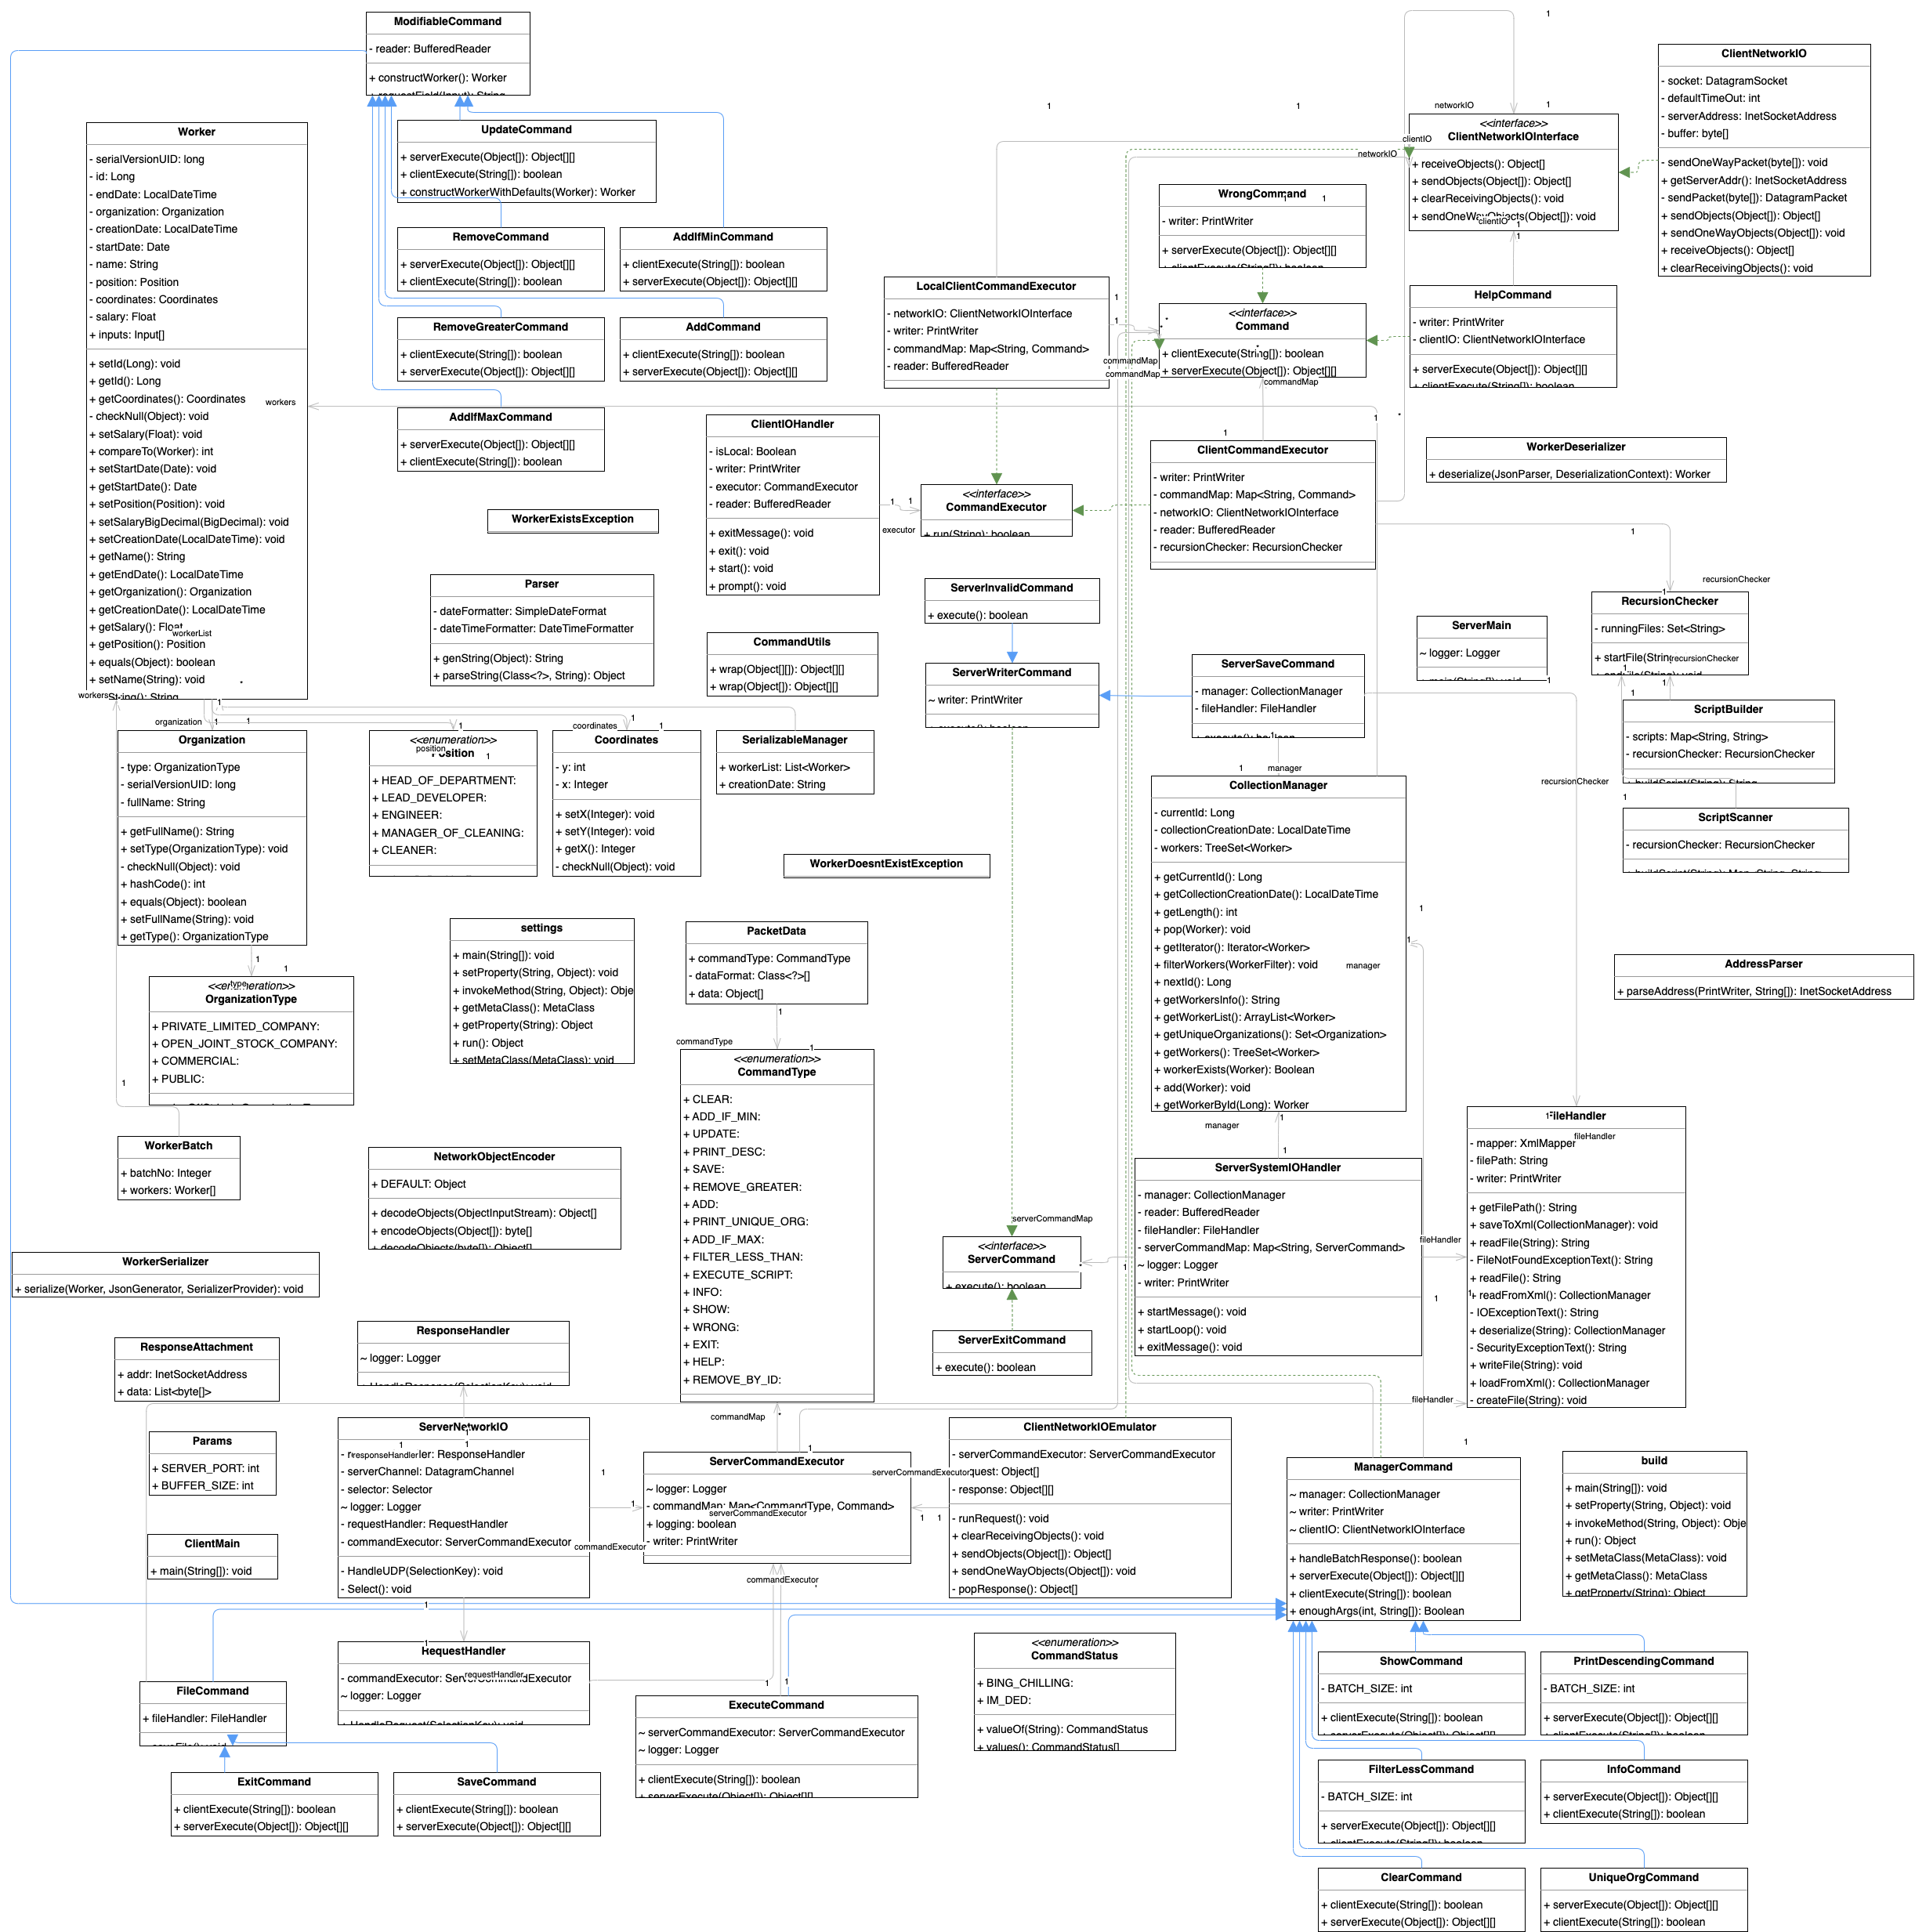
\includegraphics[width=\columnwidth]{imgs/lab6_graph.png}

\section{Исходный код программы}
https://github.com/Ne0Ment/ITMO-proga/blob/main/lab6/src/

\section{Вывод программы}
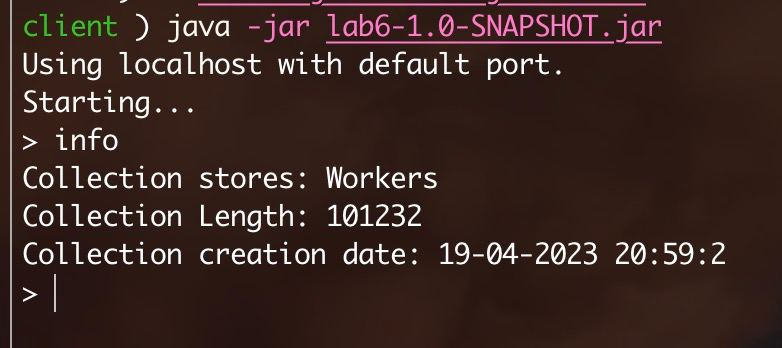
\includegraphics[width=\columnwidth]{imgs/lab6_out.jpg}

\section{Вывод}
В ходе выполнения лабораторной работы я научился использовать сетевую функицональность Java, в том числе UDP, Datagram, DatagramChannel, а также изучил основы функционального программирования.\\

\end{document}